\chapter{Classificazione delle applicazioni mobili}
\section{Introduzione}
In questo capitolo si procede all'esplorazione delle varie metodologie di sviluppo di applicazioni nate in questo ultimo decennio. Si vanno ad analizzare pregi, difetti e peculiarità di ogni approccio. Inoltre, si va a considerare quali possono essere i contesti d'uso in cui è preferibile utilizzare una metodologia rispetto ad un'altra.

\section{Native}
Nel corso di questo ultimo decennio, lo sviluppo di applicazioni \textit{mobile} ha subito una profonda trasformazione ed evoluzione. Inizialmente lo sviluppo di applicazioni era possibile soltanto con i linguaggi di programmazione supportati dal sistema operativo. Di conseguenza era necessario conoscere le varie piattaforme (\textbf{Android}, \textbf{iOS} e \textbf{Windows Phone} sono i principali sistemi operativi per mobile che hanno caratterizzato questo mercato in questo decennio). Inoltre, per sviluppare applicazioni che potessero utilizzare appieno sia l'hardware che il software del dispositivo, era ed è tuttora necessario avere un'approfondita conoscenza di tutti i sistemi operativi su cui si vuole distribuire la propria applicazione. 

Al giorno d'oggi i due competitor che coprono la quasi totalità del mercato mobile sono Android e iOS \cite{statistiche_os_mobile}. Essendo progettate per uno specifico sistema operativo, queste applicazioni sono ottimizzate e riescono a garantire delle prestazioni ottimali. Il linguaggio di programmazione utilizzato offre una serie di funzionalità e librerie che permettono il completo accesso alla componentistica hardware del dispositivo (ad esempio, l'accesso ai sensori).

Possiamo osservare le considerazioni appena fatte da un punto di vista economico: se si vuole sviluppare un'applicazione e la si vuole distribuire sia su dispositivi Android che iOS, l'azienda dovrà assumere (almeno) uno sviluppatore per ogni sistema operativo. Più aumenta la complessità dell'applicazione, più persone dovranno essere aggiunte ai due team di sviluppo. Concettualmente, è necessario sviluppare \textit{due codici sorgenti} della \textit{medesima applicazione} per poterla distribuire su due \textit{store} differenti (\textit{Play Store} per Android e \textit{App Store} per iOS). Questo comporta ad assumere diversi sviluppatori per realizzare quella che è concettualmente una singola applicazione.

Da un punto di vista tecnico, lo sviluppo della medesima applicazione da parte di due team che operano su ambienti differenti, portano a numerose difficoltà a livello di progettazione dell'applicazione e a livello organizzativo. Ad esempio, a parità di conoscenze ed esperienza dei singoli componenti dei team di sviluppo sulla piattaforma in cui operano (la conoscenza delle \textit{hard skills}), l'introduzione di una nuova funzionalità può risultare semplice da sviluppare per un team, ma può diventare fonte di difficoltà per l'altro team. Questo può provocare dei rallentamenti nel rilascio della nuova funzionalità o può generare delle \textit{asimmetrie} tra le due applicazioni, ovvero, una funzionalità può essere disponibile per un sistema operativo ma non nell'altro.

Volendo riassumere in punti i vantaggi e gli svantaggi dell'approccio nativo:
\begin{enumerate}
	\item I vantaggi sono:
	\begin{enumerate}
		\item Le applicazioni native sono più veloci e più affidabili in termini di prestazioni. In generale sono più efficienti avendo a disposizione l'accesso alle risorse del dispositivo rispetto ad altri approcci di sviluppo;
		\item Utilizzano l'interfaccia utente del dispositivo nativo, offrendo agli utenti un'esperienza più ottimizzata;
		\item Avendo il pieno accesso all'hardware del dispositivo, può essere utilizzata un'ampia gamma di funzionalità, come ad esempio il giroscopio, la bussola, il Bluetooth, la posizione GPS ed altro ancora.
	\end{enumerate}

	\item Gli svantaggi sono:
	\begin{enumerate}
		\item La non portabilità: una volta realizzata un'applicazione per uno specifico sistema operativo, questa non può essere utilizzata in altre piattaforme. Questo implica il bisogno di assumere diversi sviluppatori con conoscenze specifiche su uno specifico sistema operativo per poter realizzare l'app. Le principali conseguenze di questo svantaggio sono l'aumento dei costi (sia in termini di tempo che economici) e la difficoltà nel manutenere l'applicazione;
		\item Simmetria dei codici sorgenti: avendo più codici sorgenti per diversi sistemi operativi, si manifesta la difficoltà di mantenere aggiornati tutti i codici sorgenti nel momento in cui si vuole rilasciare una nuova funzionalità;
		\item Ogni aggiornamento dell'applicazione deve essere scaricato manualmente dall'utente tramite l'apposito store;
		\item L'applicazione contribuisce ad occupare lo spazio di memoria del dispositivo.
	\end{enumerate}

\end{enumerate}

In origine, l'unico linguaggio permesso per la realizzazione di applicazioni per Android era \textbf{Java}. Oggi è possibile creare delle applicazioni anche con \textbf{Kotlin}. Analogamente, per quanto riguarda iOS all'inizio era permesso soltanto il linguaggio \textbf{Objective-C}, mentre, oggi è possibile sviluppare app anche con \textbf{Swift}, un linguaggio sviluppato appositamente dalla casa madre per i suoi dispositivi.

\section{Web App}
Tutte le considerazioni fatte a riguardo l'approccio nativo hanno portato allo sviluppo di applicazioni Web che fossero \textbf{mobile friendly}, ovvero, che potessero essere facilmente utilizzate anche da smartphone. L'intento principale è quello di sviluppare un'applicazione indipendentemente dalla piattaforma su cui verrà ospitata, ovvero, tramite l'utilizzo del \textit{browser}, software installabile in qualsiasi dispositivo. Nonostante il nome possa trarre in inganno, queste applicazioni vengono denominate \textit{Web app}. Le Web app non sono delle vere e proprie app, ma si cerca di rendere \textbf{responsive} il sito web, ovvero, di rendere il sito \textit{mobile friendly}. Per \textit{mobile friendly} si intende che la Web app deve avere un'interfaccia grafica che si adatti alle dimensioni dello schermo in maniera dinamica ed automatica. Sviluppando secondo questa concezione, è sufficiente implementare un unico codice sorgente per distribuire l'applicazione su qualsiasi dispositivo mobile e desktop (\textit{Write once use everywhere}). L'utilizzo di queste applicazioni non comportano ad alcuna installazione e di conseguenza non incideranno sullo spazio di memoria del dispositivo. L'applicazione è sempre aggiornata all'ultima versione perchè è sempre richiesta la connessione ad Internet per poterla usufruire. I costi per lo sviluppo sono abbattuti dal momento che il team che ha realizzato il sito web può anche sviluppare la versione per mobile, senza i problemi di distribuzione su piattaforme diverse.

Tuttavia non è possibile utilizzare appieno le risorse hardware e software che offre il dispositivo e di conseguenza l'ambito di applicazione di questa metodologia di sviluppo risulta essere limitato. 
L'interfaccia grafica e l'esperienza utente sono di basso livello e le applicazioni di questo genere sono molto limitate in termini di funzionalità.

Per realizzare queste applicazioni vengono utilizzati i linguaggi di programmazione per lo sviluppo di siti Web, ovvero, HTML, CSS, JavaScript e PHP.

In conclusione a questa sezione, possiamo notare che l'approccio nativo e quello delle Web app siano \textit{diametralmente opposti}.

\section{Progressive Web App}
Un'evoluzione delle Web app sono le \textbf{Progressive Web App (PWA)}. Sono molto simili alle Web app, ovvero, mantengono alcune caratteristiche come la possibilità di sviluppare un unico codice sorgente per distribuire l'applicazione su qualsiasi dispositivo e la necessità di non doverla installare. Tuttavia, permettono di ricevere delle \textit{notifiche push} e possono essere utilizzate anche in assenza di connessione ad Internet. Le PWA si appoggiano comunque al browser del dispositivo e quindi presentano le medesime limitazioni in termini di accessibilità delle Web app. Ad esempio, è possibile utilizzare il servizio GPS, ma non è possibile accedere alla fotocamera.

Per realizzare queste applicazioni vengono utilizzati i classici linguaggi per lo sviluppo di siti Web, ovvero, HTML, CSS e JavaScript. Per quanto riguarda i framework più comuni vi sono \textbf{Angular} (Google) e \textbf{ReactJS} (Facebook).

\section{Hybrid}
Le \textbf{app ibride} si pongono come un'evoluzione delle Web app e delle PWA e tentano di congiungere i vantaggi dello sviluppo nativo e delle PWA. Vengono create con i medesimi linguaggi per lo sviluppo Web, ma per funzionare necessitano l'installazione di un software sul device (\textit{engine}). Questo software è uno strato che si interpone tra il dispositivo e l'applicazione ed è necessario per l'esecuzione del codice. L'engine permette di utilizzare in maniera più efficiente e profonda l'hardware del device, oltre ad effettuare il \textit{rendering} della grafica. Ad esempio, è possibile realizzare applicazioni che facciano uso di sensori come l'accelerometro e il giroscopio.

Nonostante questi vantaggi, alcune funzionalità non possono essere realizzate e le prestazioni generali (compresa la \textit{User Experience}) sono nettamente inferiori rispetto alle app native. Inoltre, rispetto alle Web app e alle PWA, queste applicazioni devono necessariamente essere pubblicate sullo store per poter essere installate sul dispositivo. 

Il vantaggio fondamentale che si può ottenere è la possibilità di produrre un unico codice sorgente, utilizzando i classici linguaggi per lo sviluppo Web. Così facendo, è possibile distribuire l'applicazione su più dispositivi possibili, abbattendo in questo modo i costi.

I framework più comuni per la realizzazione di app ibride sono \textbf{Ionic} e \textbf{Apache Cordova}.

\begin{figure}
	\begin{center}
		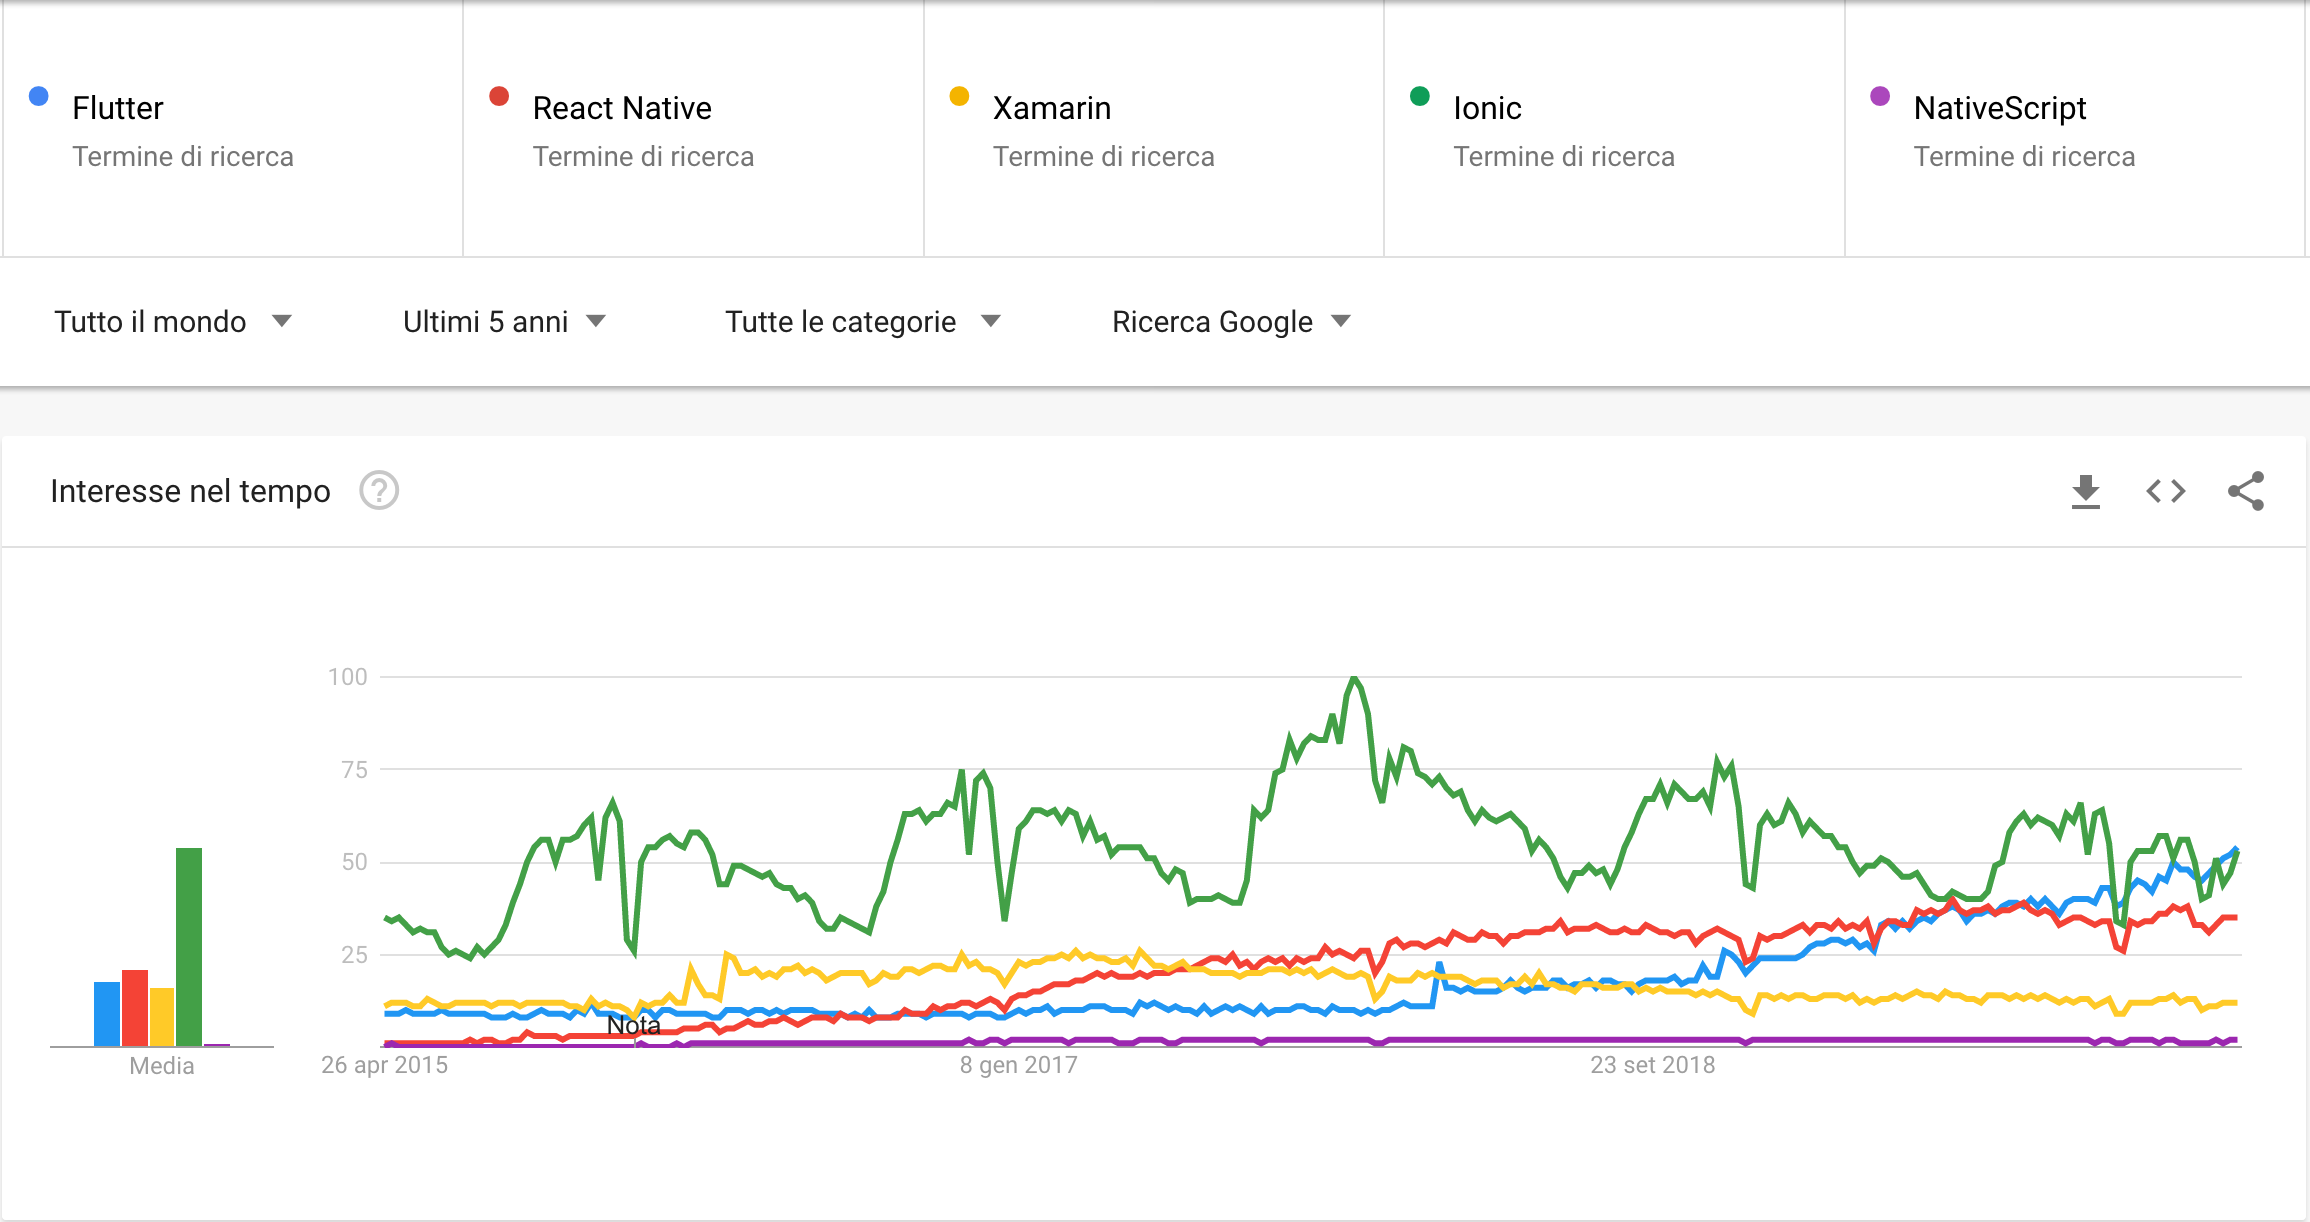
\includegraphics[scale=0.35]{google_trends}
		\caption[Google Trends - Framework Cross-Paltform]{Trends dei framework cross-platform su Google Trends \cite{google_trends}}
		\label{figura:google_trends}
	\end{center}
\end{figure}

\section{Cross-Platform}
Le applicazioni \textbf{cross-platform}, anche dette \textit{platform-independent}, sono applicazioni installabili su dispositivi con sistemi operativi differenti, senza la necessità di produrre un codice sorgente per ogni piattaforma. Sulla base di quanto appena detto, queste applicazioni possono essere confuse per applicazioni ibride, tuttavia hanno delle caratteristiche peculiari che le differenziano. In particolare, le app cross-platform utilizzano un \textit{render engine} nativo che le permette di collegare il codice sorgente direttamente ai componenti nativi dei dispositivi. Così facendo, si aumentano notevolmente le prestazioni ed è possibile sfruttare meglio le risorse hardware rispetto alle applicazioni ibride. Le app ibride fanno uso, invece, di un render creato ad \textit{hoc}. È comunque importante ricordare che soltanto le applicazioni native possono ottenere delle prestazioni ottimali: tutte le altre metodologie di sviluppo cercano di avvicinarsi ma non raggiungono i livelli di un approccio nativo.

In un'applicazione cross-platform è possibile implementare delle funzionalità particolari ed è possibile avere un interfaccia grafica fluida e reattiva, comparabile ad un'app nativa. Questo è l'approccio che più si avvicina alle applicazioni native e pertanto può essere considerata la metodologia più opportuna se si vuole sviluppare un'applicazione senza dover assumere due team di sviluppo differenti e senza sprecare le risorse economiche dell'azienda.

I framework più popolare in questo ambito di sviluppo sono \textbf{React Native} (Facebook), \textbf{Xamarin} (Microsoft) e \textbf{Flutter} (Google).

I linguaggi utilizzati variano da framework a framework: React Native utilizza \textit{JavaScript}, Xamarin permette di scrivere codice in \textit{C\#} (linguaggio proprietario di Microsoft) e Flutter in \textit{Dart} (linguaggio proprietario di Google).

\begin{figure}
	\begin{center}
		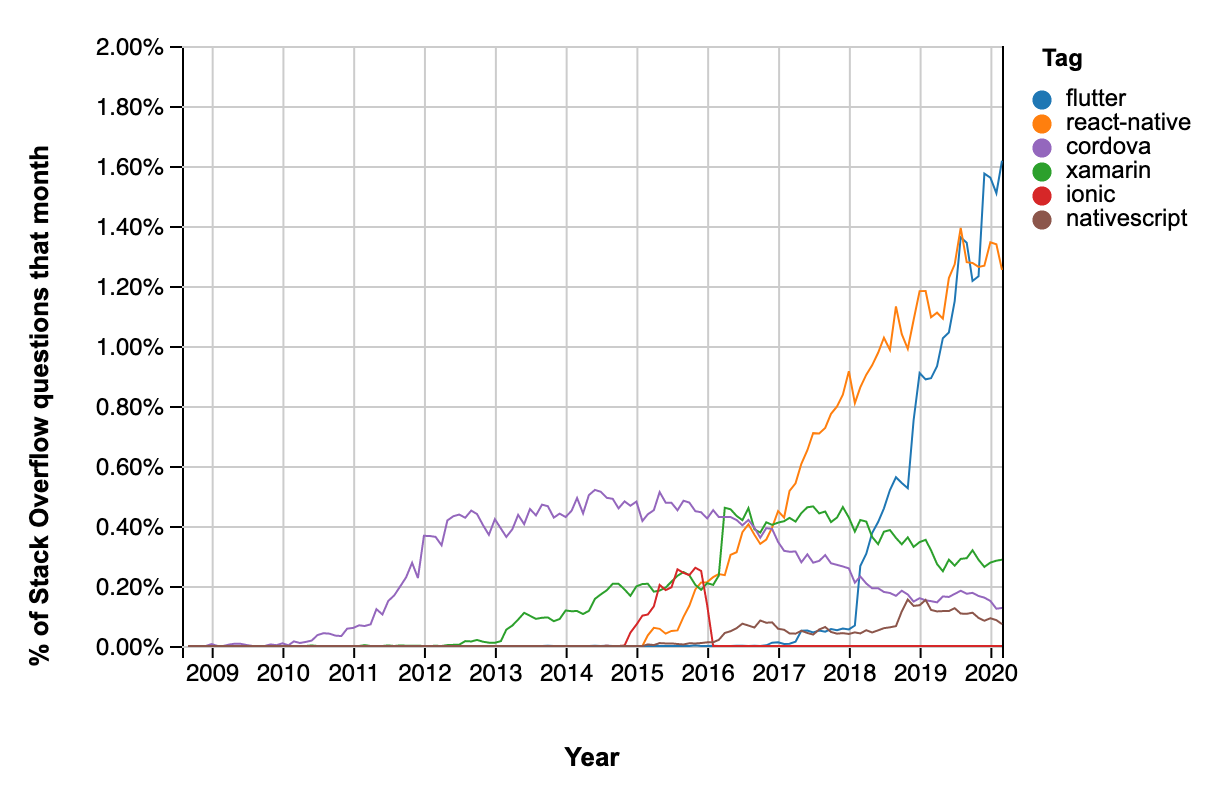
\includegraphics[scale=0.6]{stackoverflow_trends}
		\caption[StackOverflow - Framework Cross-Paltform]{Trends dei framework cross-platform su StackOverflow \cite{stackoverflow_trends}}
		\label{figura:stackoverflow_trends}
	\end{center}
\end{figure}

\section{Considerazioni}
\begin{figure}
	\begin{center}
		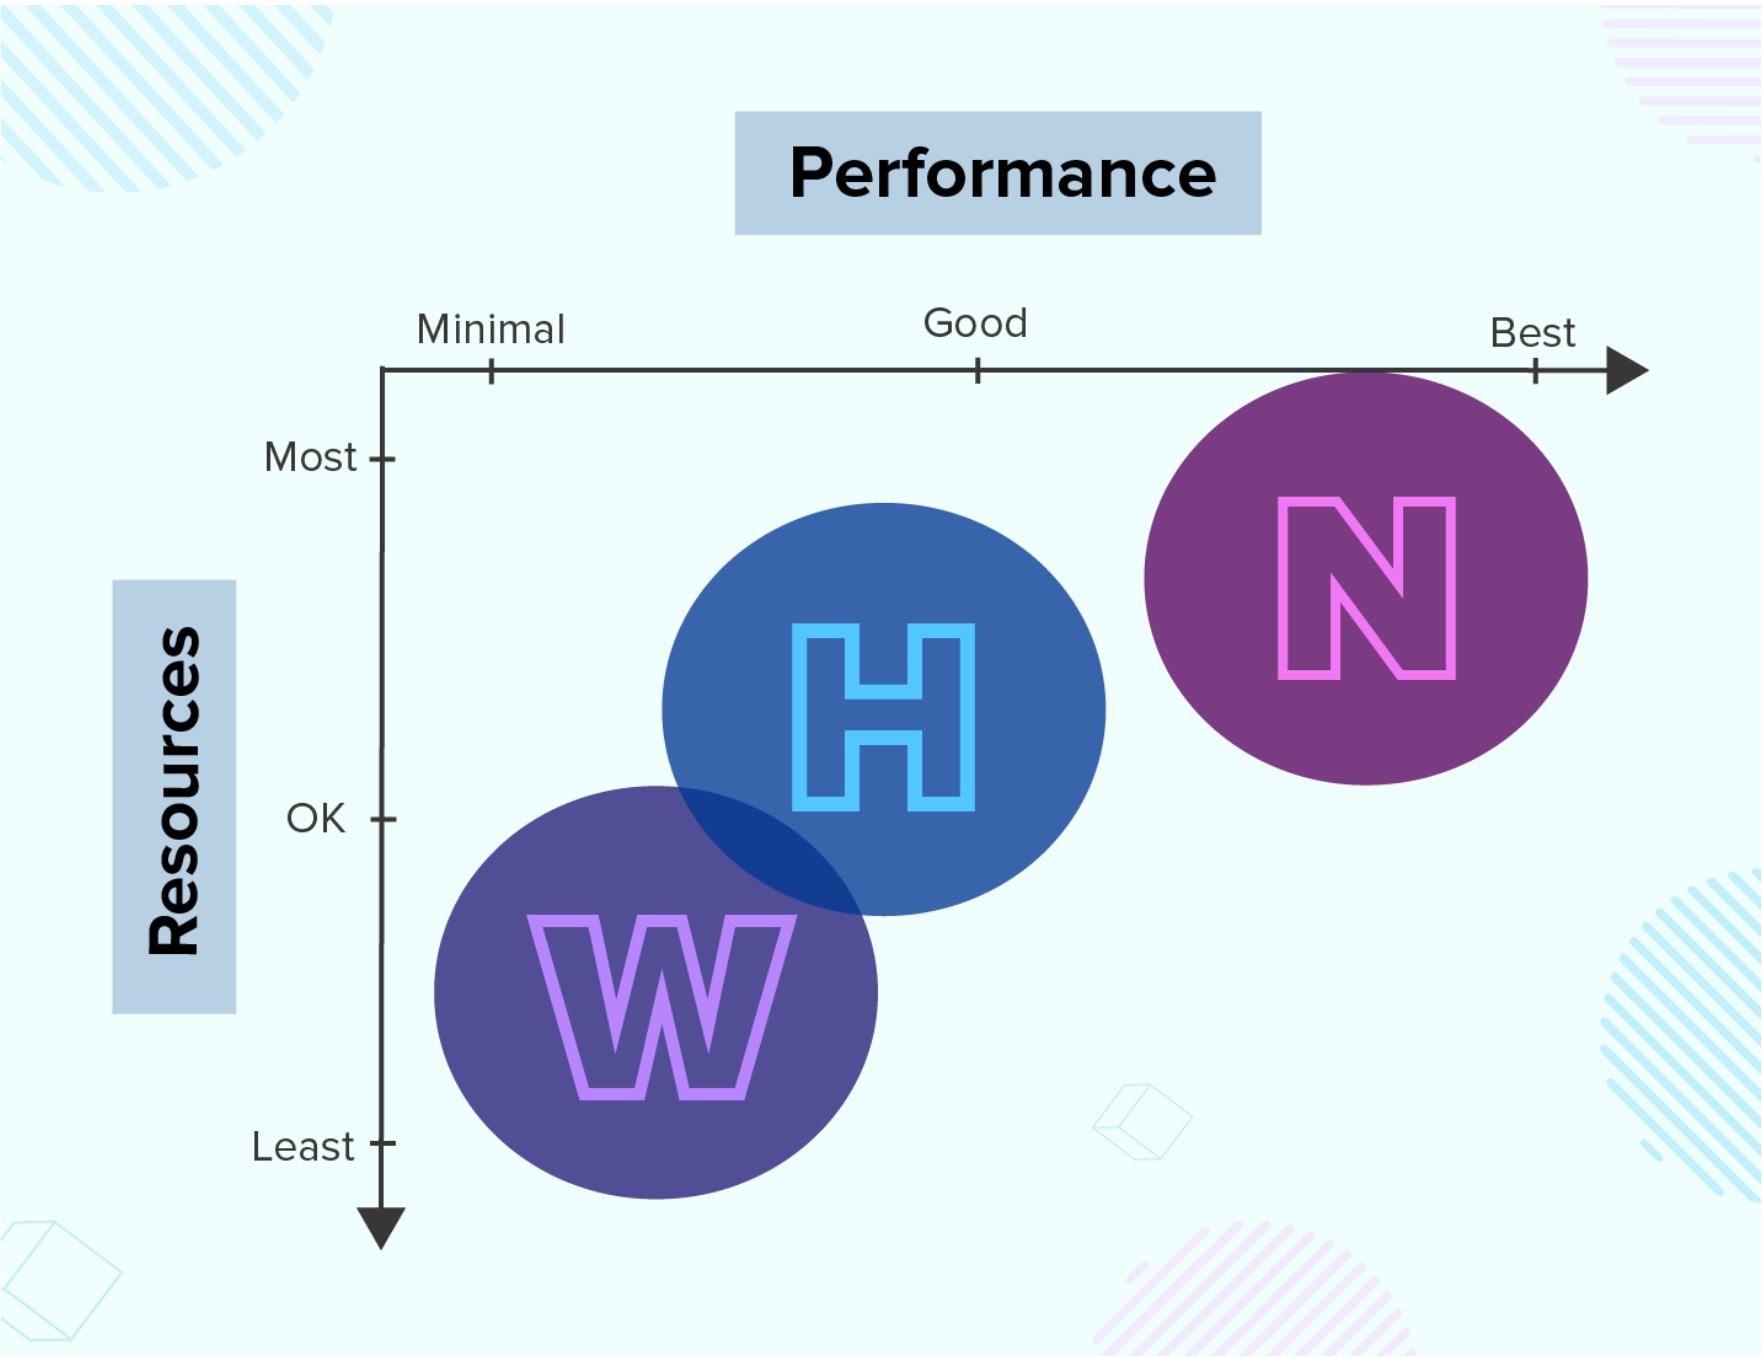
\includegraphics[scale=0.3]{native_hybrid_web}
		\caption[Confronto Native, Hyrbid, Web]{Confronto fra app Native, Hyrbid, Web \cite{grafico_native_hybrid_web}.}
		\label{figura:native_hybrid_web}
	\end{center}
\end{figure}

La decisione di esporre le varie metodologie di sviluppo non è stata presa in modo casuale. Si è voluto mettere in evidenza fin dall'inizio i due approcci in antitesi tra loro, ovvero, le \textit{applicazioni native} e le \textit{Web app}. A partire dalle Web app, si è proceduti verso un progressivo avvicinamento alle applicazioni native, pur tenendo conto che tutte le metodologie presentate, permettono di sviluppare un'app per più sistemi operativi con un unico codice sorgente. In questo modo si è proceduti ad illustrare tutte le possibilità offerte dal mercato per lo sviluppo di applicazioni mobili, considerando aspetti tecnici ed economici.

Dall'analisi effettuata, si possono suddividere gli approcci descritti principalmente in due categorie: \textit{applicazioni native} e \textit{applicazioni multipiattaforma}. Web app, PWA, Hybrid app e Cross-Platform app seguono la filosofia \textbf{\textit{"Write once use everywhere"}} e \textbf{\textit{"Learn once apply everywhere"}}, ovvero, la possibilità di realizzare un unico codice sorgente per distribuire l'applicazione su qualsiasi piattaforma, riutilizzando dei linguaggi di programmazione già esistenti, senza dover imparare uno specifico linguaggio per ogni singolo framework. I principi fondanti di questa categoria di approcci sono:

\begin{enumerate}
	\item \textbf{Manutenibilità}: è sicuramente il vantaggio più importante in termini di tempo e di risorse economiche risparmiate nel processo di realizzazione di un’applicazione. Sviluppando infatti un unico codice per l’applicazione, le attività di manutenzione, correzione e identificazione di eventuali malfunzionamenti risultano essere più veloci;
	\item \textbf{Rapidità di sviluppo}: i tempi di realizzazione, dovendo scrivere un unico codice per tutte le piattaforme, si riducono notevolmente.
\end{enumerate}

In conclusione, possiamo considerare che lo sviluppo di Web app (incluse le PWA) fanno un uso minimale delle risorse offerte dal dispositivo, mentre le applicazioni native fanno un largo uso delle risorse disponibili (Figura 3.3). Le applicazioni ibride si pongono come un compromesso tra la complessità delle applicazioni native e le forti limitazioni delle Web app. Le app cross-platform possono essere collocate vicino alle app native, sia per quanto riguarda la possibilità di utilizzare le risorse del dispositivo e sia dal punto di vista delle prestazioni, ma anche vicino alle Web app per quanto riguarda la semplicità di sviluppo e dell'uso di linguaggi comuni alla programmazione Web (Figura 3.3).

\section{Criteri per la scelta dell'approccio di sviluppo}
In questa breve sezione si prendono in considerazione alcuni degli aspetti e delle motivazioni che possono portare a scegliere un determinato approccio rispetto ad un altro \cite{considerazioni_native_hybrid_cross_platform}.

\subsection{Risorse economiche a disposizione}
Quando si parla dello sviluppo di un'applicazione, un aspetto fondamentale e rilevante è l'\textit{aspetto economico}. Nel contesto di una piccola azienda o di una \textit{startup}, di solito sono disponibili pochi fondi per la realizzazione dell'applicazione. Pertanto, lo sviluppo nativo non è quello consigliato in quanto è necessario trovare uno sviluppatore che sia in grado di programmare sia per Android che per iOS o costruire due team di sviluppo per ogni sistema operativo. È evidente che questo approccio è il più \textit{dispendioso}. In queste situazioni è molto importante concentrare tutti gli sforzi su un'unica piattaforma per ottenere un prodotto finale completo.

Se l'aspetto economico non è un problema, non è necessario comunque sviluppare delle app native. Ad esempio, se un'azienda ha già degli sviluppatori molto esperti in JavaScript, risulta inefficiente non sfruttare le potenzialità di questo team anche per lo sviluppo di un'applicazione per dispositivi mobile. Sopratutto, quando si hanno dei tempi stretti per la realizzazione del prodotto e per la consegna, è consigliato di sfruttare appieno le risorse già presenti nell'ambiente aziendale, senza dover procedere con dei colloqui per assumere altri sviluppatori.

\subsection{Time-to-market e copertura del mercato (reach)}
La creazione di un'applicazione nativa richiede molto più tempo rispetto allo sviluppo di app ibride o PWA. Le tempistiche dettate dal mercato (\textbf{time-to-market}) influenzano le scelte anche di questo genere. Pertanto se si vuole realizzare un prodotto funzionante prima di un \textit{competitor}, è necessario prendere in considerazione anche le vie alternative allo sviluppo nativo. Una volta che il prodotto è stato sufficientemente accettato dal mercato (quando ha superato la cosiddetta \textit{massa critica}), allora si può pensare di ristrutturare l'applicazione e di scegliere altri approcci per gli sviluppi futuri.

Se parliamo in termini di \textbf{reach}, ovvero, di copertura del mercato con il proprio prodotto, è preferibile che l'applicazione possa essere distribuita nel più breve tempo possibile e su più \textit{marketplace} possibili. Questo aspetto invita ad adottare un approccio ibrido o cross-platform, per poter generare con un unico codice sorgente, due versioni dell'app pronte per entrambi gli store.

\subsection{Performance dell'applicazione}
Se le prestazioni sono un fattore fondamentale ed un requisito indispensabile, l'approccio nativo è quello migliore di tutti. Tutti gli altri approcci introducono dell'\textit{overhead}: si pensi ad esempio al bridge JavaScript di React Native per poter utilizzare gli elementi grafici nativi. Un'applicazione nativa ha il pieno accesso alle risorse hardware e software del dispositivo e in questo modo è possibile operare con precisione ed in profondità per ottenere dei vantaggi in termini di prestazioni e di ottimizzazioni.

\subsection{User Experience e interfaccia grafica}
Secondo una statistica del 2018 \cite{tasso_di_abbandono_app}, quasi \textit{una persona su tre} abbandona l'applicazione dopo la prima esperienza. Questo dato stimola la riflessione riguardo alla \textbf{UX} (\textbf{User Experience}) e la \textbf{UI} (\textbf{User Interface}), aspetti fondamentali che devono essere curati se si vuole mantenere una buona \textit{retention} dell'utente nell'applicazione. Le applicazioni native permettono meglio di qualunque altro approccio di realizzare delle animazioni dinamiche e degli scorrimenti fluidi. Dopo le applicazioni native, le app cross-platform sono quelle in grado di riprodurre al meglio una UX vicina a quella che può essere implementata in ambiente nativo. Per quanto riguarda le applicazioni ibride e Web, l'esperienza va a mano a mano a degradarsi.

\subsection{Funzionalità}
Se l'applicazione che deve essere prodotta deve avere delle particolari funzionalità o deve utilizzare determinati sensori, l'approccio migliore è quello nativo perché è possibile accedere completamente a tutte le risorse del dispositivo. A partire dalle applicazioni cross-platform fino alle Web app, la possibilità di interagire con determinati componenti hardware installati nel dispositivo risulta essere sempre più difficile se non impossibile da attuare.

\section{Motivazione della scelta di un framework cross-platform}
Le motivazioni che mi hanno portato a scegliere di utilizzare un approccio cross-platform sono principalmente dovute per ragioni intrinseche del progetto da sviluppare. L'applicazione che deve essere realizzata necessita di visualizzare in \textit{tempo reale} dei dati provenienti da una socket. In particolare si deve tener conto che l'applicazione debba essere \textit{reattiva}. Inoltre si vuole rendere l'applicazione disponibile per più dispositivi mobili, con sistemi operativi differenti. Sulla base di queste considerazioni, l'approccio più plausibile da utilizzare è l'approccio cross-platform, in quanto:
\begin{enumerate}
	\item Permette di creare un'unico codice sorgente per distribuire l'applicazione sia su Android che su iOS;
	\item È l'approccio che più si avvicina a quello nativo, in termini di prestazioni e di accessibilità alla componentistica hardware del dispositivo;
	\item È possibile realizzare un'interfaccia grafica che sia fluida e reattiva, grazie proprio alla maggior vicinanza con l'hardware del device.
\end{enumerate}

La scelta della metodologia cross-platform rappresenta quindi un \textit{trade-off} tra la possibilità di sviluppare un unico codice sorgente sia per Android che per iOS e le prestazioni dell'applicazione.